\section{Recorrido por Perspectiva de Cuentas Contables}

\begin{enumerate}

\item
    \begin{minipage}[t]{\linewidth}
        Ingresar a  \url{https://mdm.somoscmi.com:8443/ebx-authentication/login?resume=/ebx-iu/ui}
        \raggedright
        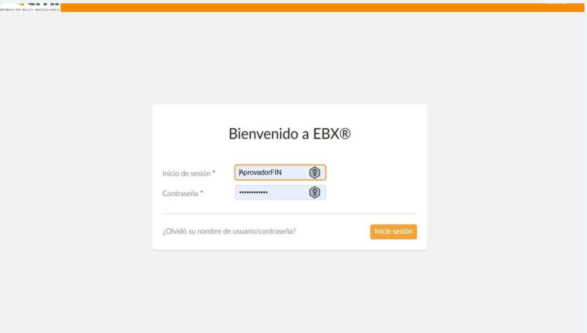
\includegraphics[width=0.8\textwidth]{RecorridoPerspectiva/ImgRecorridoPerspectiva/RP01.png}

    \end{minipage}

\item
    \begin{minipage}[t]{\linewidth}
        Click "Inicie sesión".
        \raggedright
        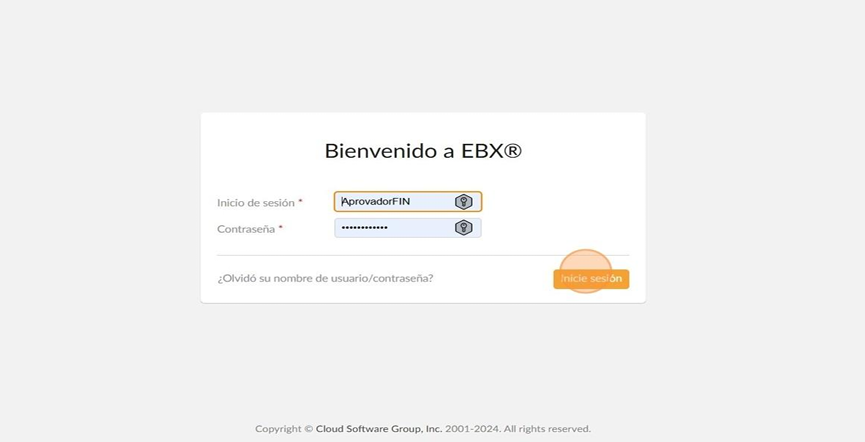
\includegraphics[width=0.8\textwidth]{RecorridoPerspectiva/ImgRecorridoPerspectiva/RP02.png}

    \end{minipage}    

\item
    \begin{minipage}[t]{\linewidth}
        Damos click "Bandeja de Entrada".
        \raggedright
        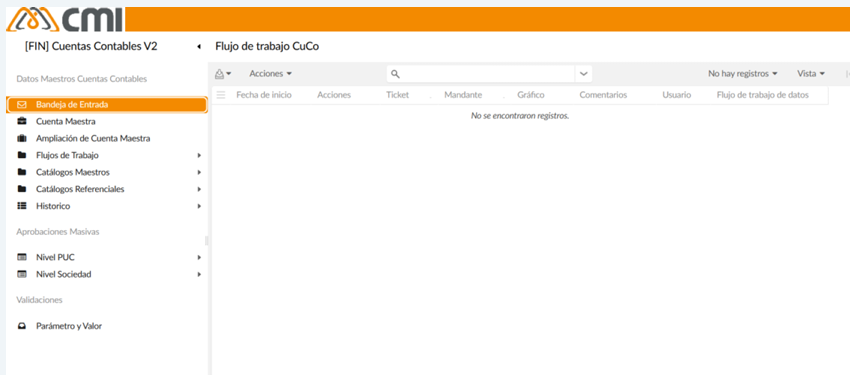
\includegraphics[width=0.8\textwidth]{RecorridoPerspectiva/ImgRecorridoPerspectiva/RP03.png}

    \end{minipage}  

\item
    \begin{minipage}[t]{\linewidth}
        Dentro de la Bandeja de Entrada están todos los flujos pendientes que tenga el usuario o el rol.

        \raggedright
        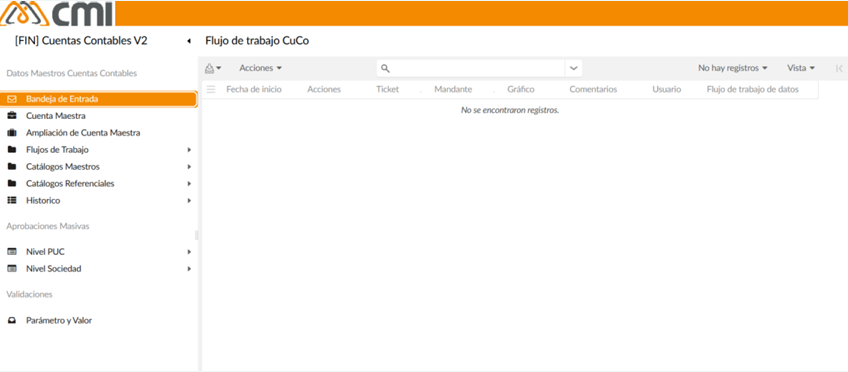
\includegraphics[width=0.8\textwidth]{RecorridoPerspectiva/ImgRecorridoPerspectiva/RP04.png}
    
    \end{minipage}  
 
\item
    \begin{minipage}[t]{\linewidth}
        Damos click "Cuenta Maestra”.
        \raggedright
        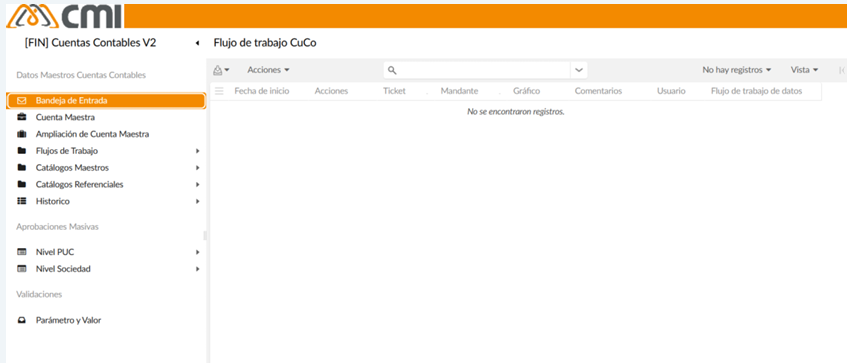
\includegraphics[width=0.8\textwidth]{RecorridoPerspectiva/ImgRecorridoPerspectiva/RP05.png}
    
    \end{minipage}

\item
    \begin{minipage}[t]{\linewidth}
        Dentro de Cuenta Maestra se encuentran las cuentas contables que se encuentran dentro SAP.
        
        Además de contar con botones que inicia el servicio creado para el dominio.
        \raggedright
        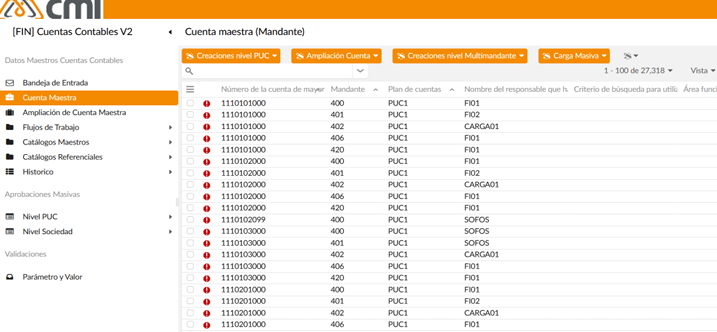
\includegraphics[width=0.8\textwidth]{RecorridoPerspectiva/ImgRecorridoPerspectiva/PR06.png}
    
    \end{minipage}      

    \item
    \begin{minipage}[t]{\linewidth}
        Damos click "Ampliación de Cuenta Maestra".
        \raggedright
        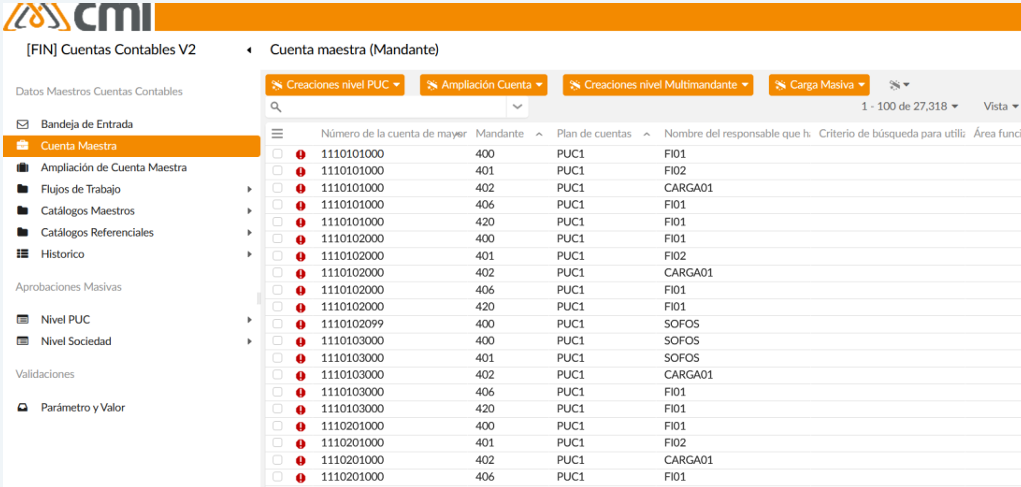
\includegraphics[width=0.8\textwidth]{RecorridoPerspectiva/ImgRecorridoPerspectiva/RP07.png}
   
    \end{minipage}   

    \item
    \begin{minipage}[t]{\linewidth}
        En Ampliación de cuenta Maestra, se encuentran las cuentas contables que están asociadas a una sociedad. 
        
        Adicional, se localizan los botones de acciones específicas para esta área.
        \raggedright
        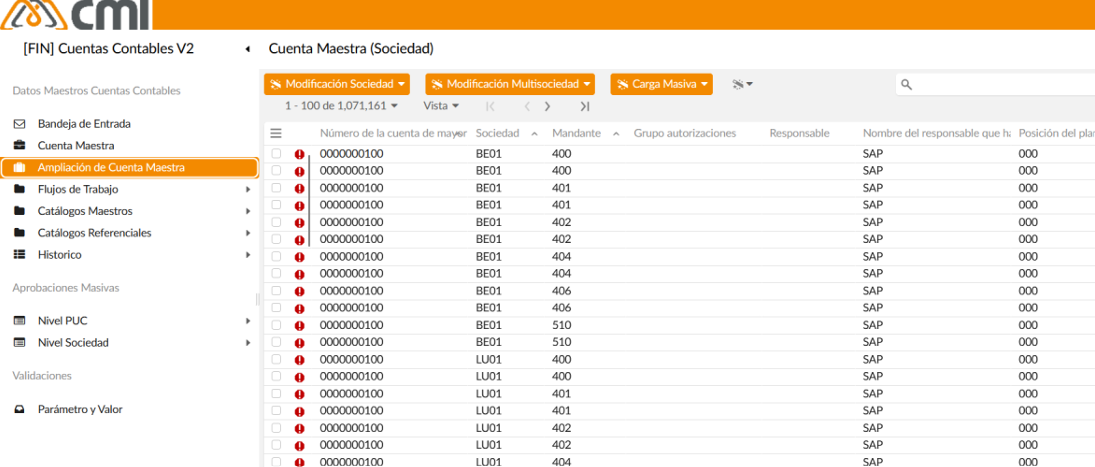
\includegraphics[width=0.8\textwidth]{RecorridoPerspectiva/ImgRecorridoPerspectiva/RP08.png}
     
    \end{minipage} 

     \item
    \begin{minipage}[t]{\linewidth}
        "Flujos de trabajo" es una lista desplegable que contiene apartados específicos para identificación de flujos de trabajo.
        
        \raggedright
        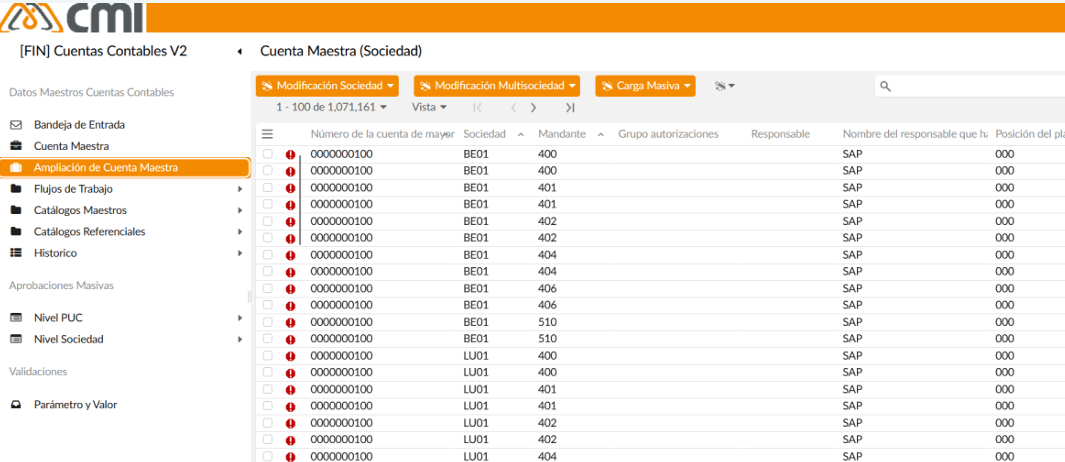
\includegraphics[width=0.8\textwidth]{RecorridoPerspectiva/ImgRecorridoPerspectiva/RP09.png}
     
    \end{minipage} 


    \item
    \begin{minipage}[t]{\linewidth}
        Dentro de "Flujos de Trabajo" se tienen 3 pestañas:
        \begin{itemize}
            \item Flujos de trabajo
            \item Flujos de trabajo activos
            \item Flujos de trabajo Completados
        \end{itemize}
        
        \raggedright
        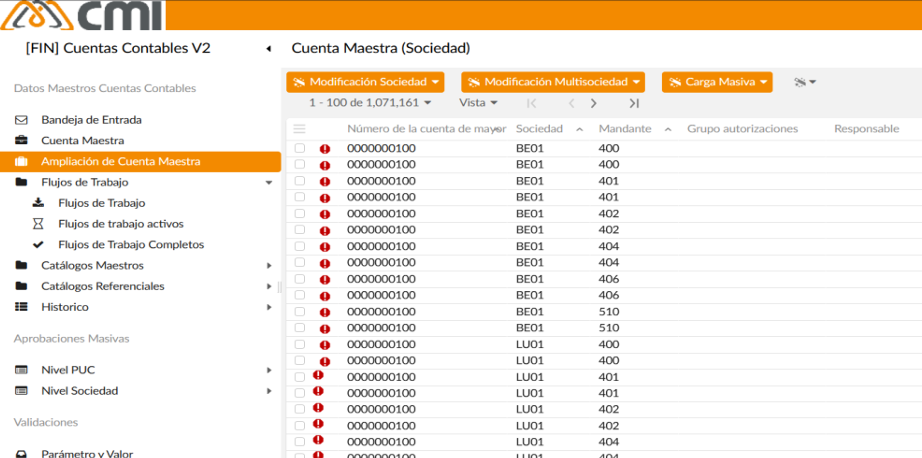
\includegraphics[width=0.8\textwidth]{RecorridoPerspectiva/ImgRecorridoPerspectiva/RP10.png}
     
    \end{minipage} 

    \item
    \begin{minipage}[t]{\linewidth}
        Dentro "Flujos de Trabajo" se tiene los flujos individuales del dominio por si es necesario una acción aislada.

        Cada flujo de trabajo tiene una etiqueta para su identificación.
        
        \raggedright
        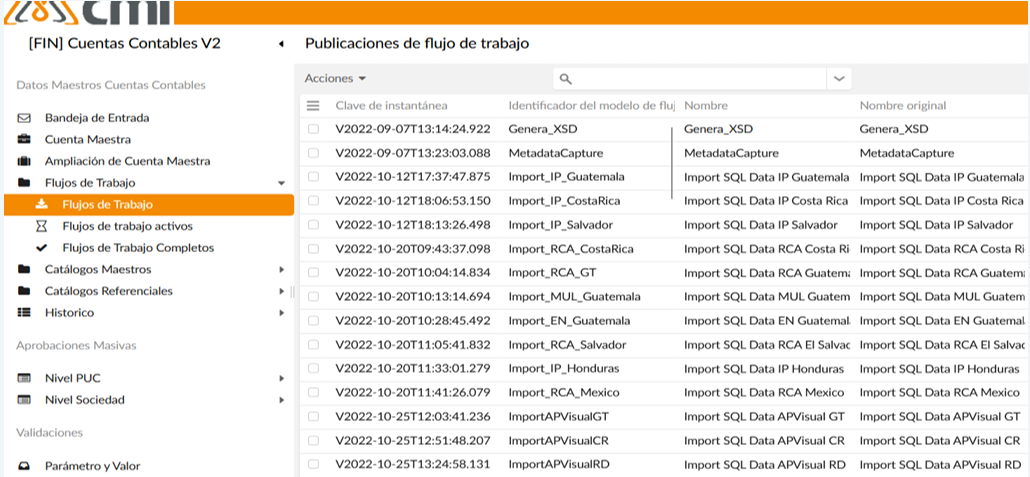
\includegraphics[width=0.8\textwidth]{RecorridoPerspectiva/ImgRecorridoPerspectiva/RP11.png}
     
    \end{minipage} 

    \item
    \begin{minipage}[t]{\linewidth}
        Si damos click en "Flujos de trabajo activos".
        
        \raggedright
        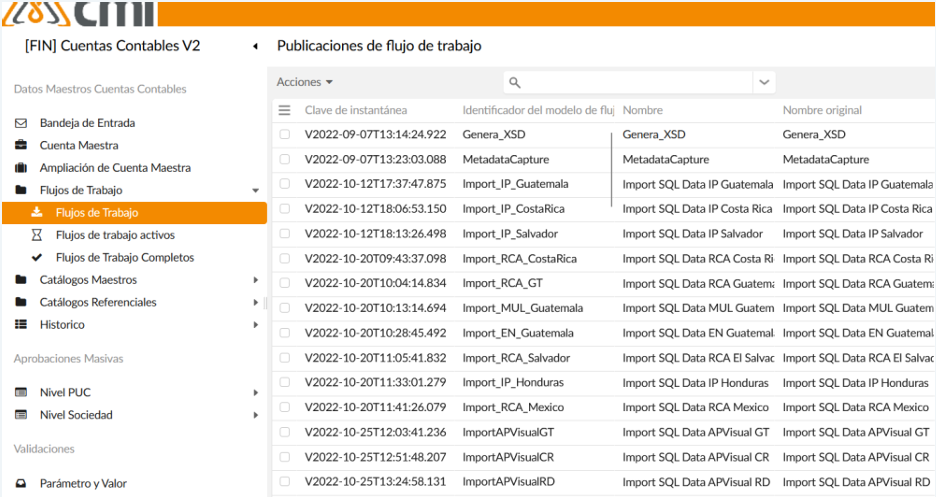
\includegraphics[width=0.8\textwidth]{RecorridoPerspectiva/ImgRecorridoPerspectiva/RP12.png}
     
    \end{minipage} 

    \item
    \begin{minipage}[t]{\linewidth}
        Dentro "Flujos de trabajo Activos" se muestra todos los flujos activos ya sea Creación / Modificación / Bloqueo / Ampliación, con su respectivo ticket y etiqueta del flujo en cuestión.
        
        \raggedright
        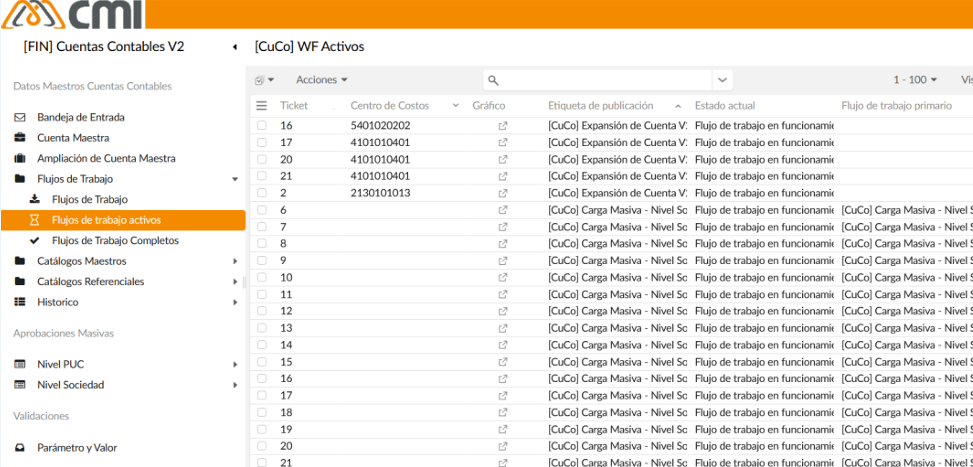
\includegraphics[width=0.8\textwidth]{RecorridoPerspectiva/ImgRecorridoPerspectiva/RP13.png}
     
    \end{minipage} 

    \item
    \begin{minipage}[t]{\linewidth}
        Si damos click en "Flujos de Trabajo Completos".
        
        \raggedright
        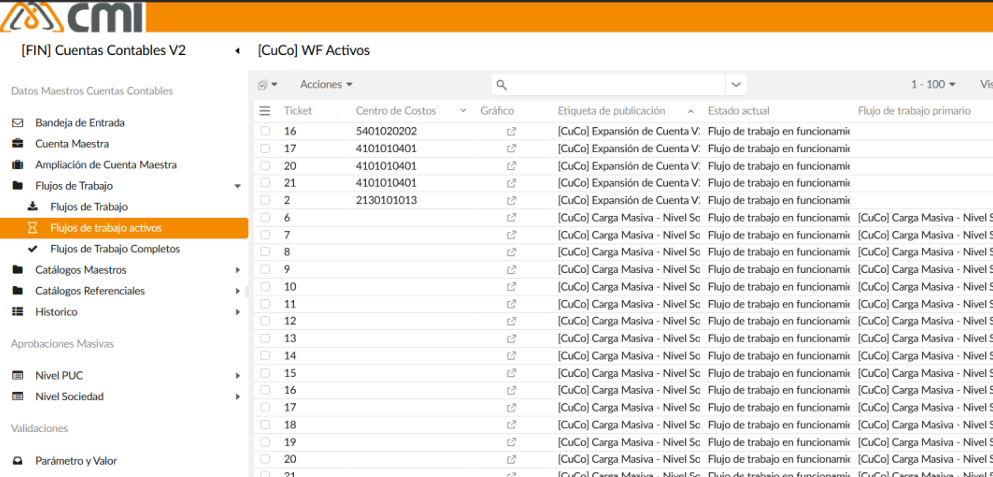
\includegraphics[width=0.8\textwidth]{RecorridoPerspectiva/ImgRecorridoPerspectiva/RP14.png}
     
    \end{minipage} 

    \item
    \begin{minipage}[t]{\linewidth}
        En "Flujos de Trabajo Completos" se encuentran todos los flujos que concluyeron para un análisis de cuales personas participaron en el flujo si es necesario.
        
        \raggedright
        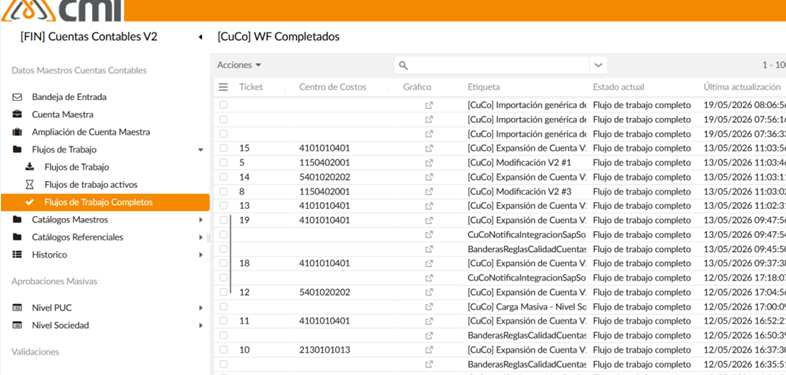
\includegraphics[width=0.8\textwidth]{RecorridoPerspectiva/ImgRecorridoPerspectiva/RP15.png}
     
    \end{minipage}
    
    \item
    \begin{minipage}[t]{\linewidth}
        "Catálogos Maestros" es otra lista que contiene todos los catálogos utilizados dentro el dominio.
        
        \raggedright
        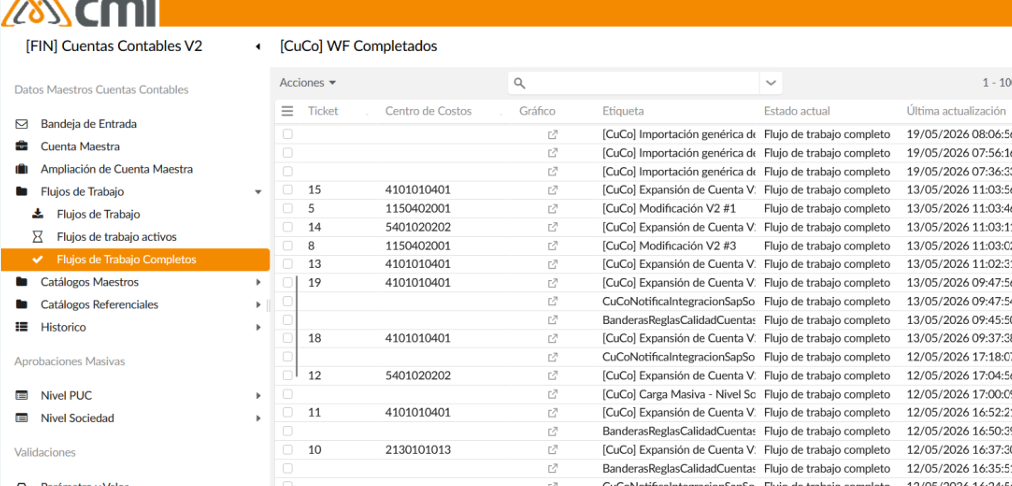
\includegraphics[width=0.8\textwidth]{RecorridoPerspectiva/ImgRecorridoPerspectiva/RP16.png}
     
    \end{minipage} 

    \item
    \begin{minipage}[t]{\linewidth}
        Damos click en "Mandante".
        
        \raggedright
        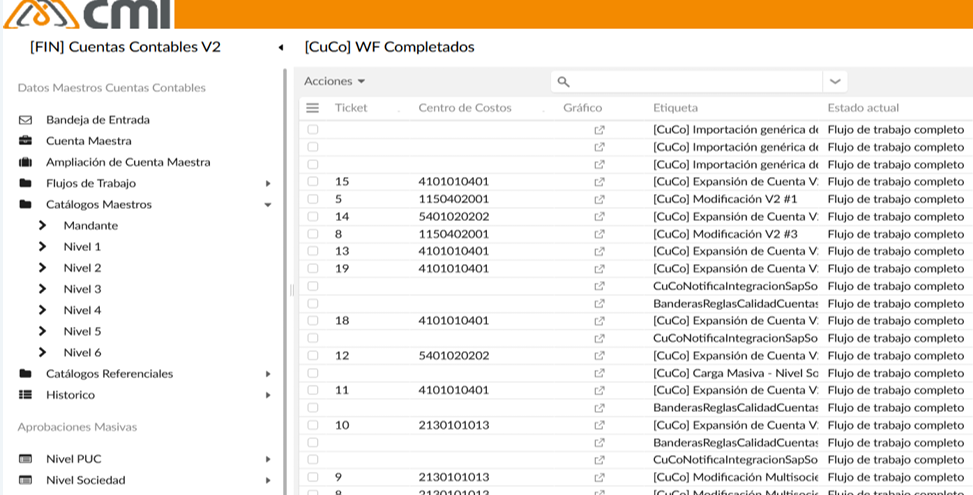
\includegraphics[width=0.8\textwidth]{RecorridoPerspectiva/ImgRecorridoPerspectiva/RP17.png}
     
    \end{minipage} 

    \item
    \begin{minipage}[t]{\linewidth}
        Se encuentran todos los mandantes asociados a los servicios desarrollados.
        
        \raggedright
        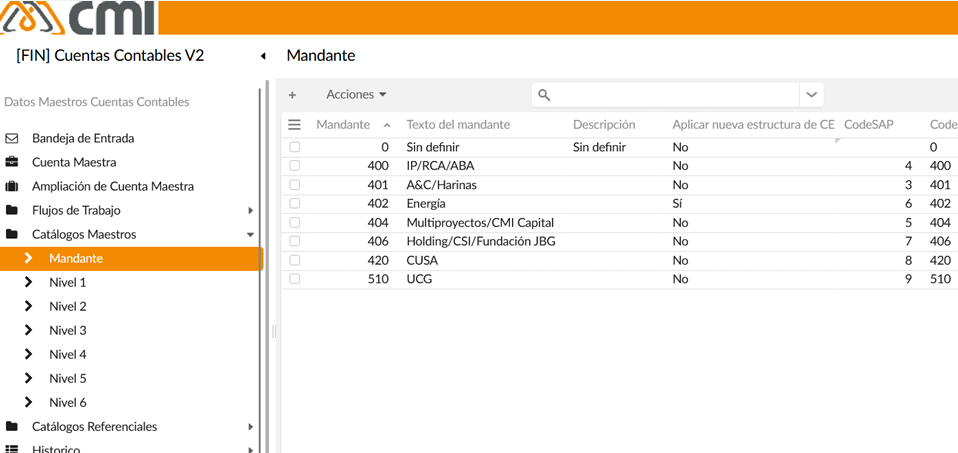
\includegraphics[width=0.8\textwidth]{RecorridoPerspectiva/ImgRecorridoPerspectiva/RP18.png}
     
    \end{minipage} 

    \item
    \begin{minipage}[t]{\linewidth}
        Si damos click en "Nivel 1".
        
        \raggedright
        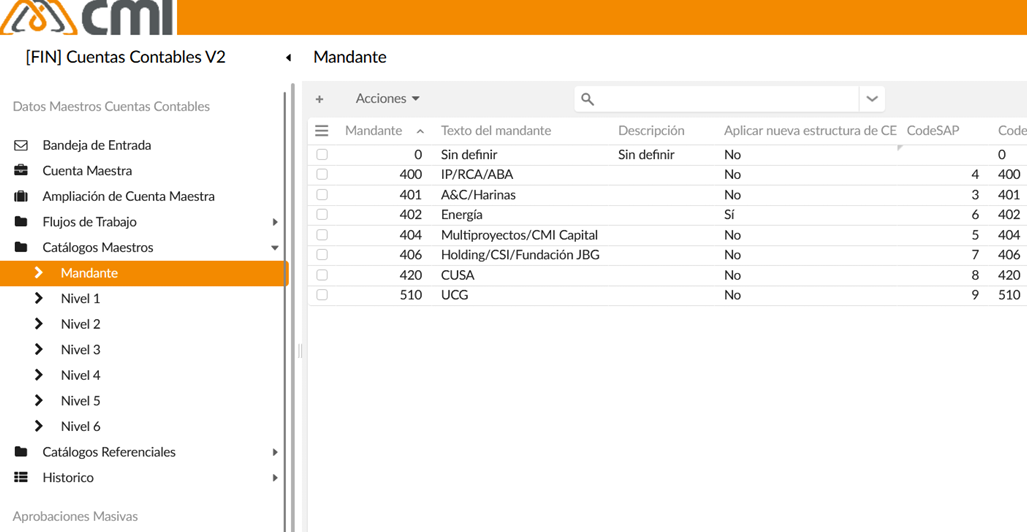
\includegraphics[width=0.8\textwidth]{RecorridoPerspectiva/ImgRecorridoPerspectiva/RP19.png}
     
    \end{minipage} 

    \item
    \begin{minipage}[t]{\linewidth}
        Dentro de "Nivel 1" se encuentra el catálogo al primer nivel de una cuenta contable.
        
        \raggedright
        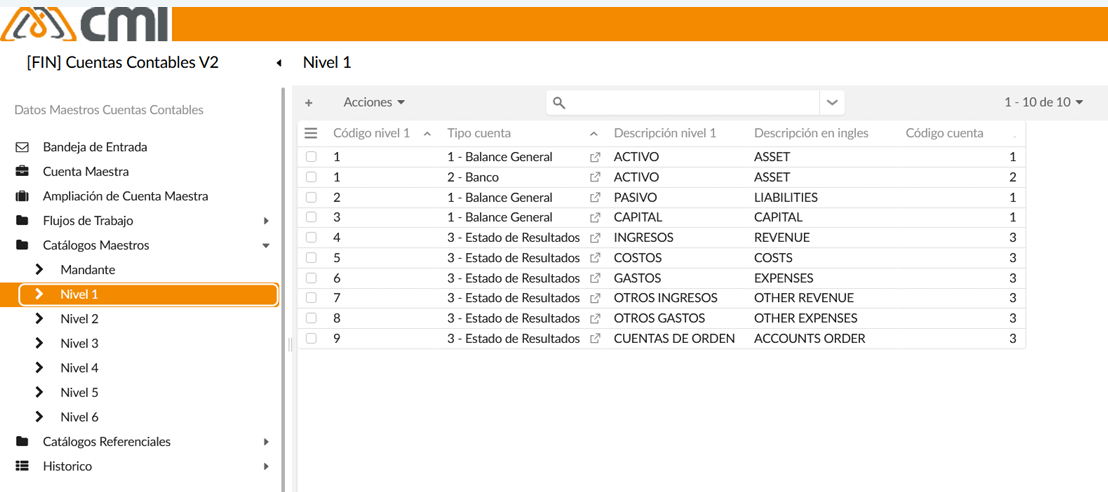
\includegraphics[width=0.8\textwidth]{RecorridoPerspectiva/ImgRecorridoPerspectiva/RP20.png}
     
    \end{minipage} 


    \item
    \begin{minipage}[t]{\linewidth}
        Dentro de "Nivel 2" se encuentra el catálogo al primer nivel de una cuenta contable.
        
        \raggedright
        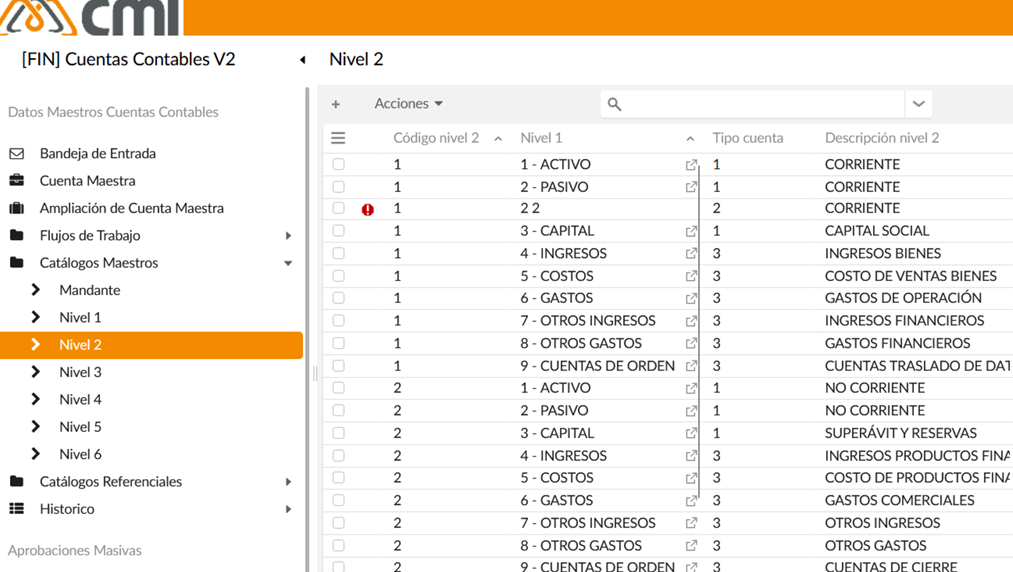
\includegraphics[width=0.8\textwidth]{RecorridoPerspectiva/ImgRecorridoPerspectiva/RP21.png}
     
    \end{minipage} 

    \item
    \begin{minipage}[t]{\linewidth}
        Dentro de "Nivel 3" se encuentra el catálogo al tercer nivel de una cuenta contable.
        
        \raggedright
        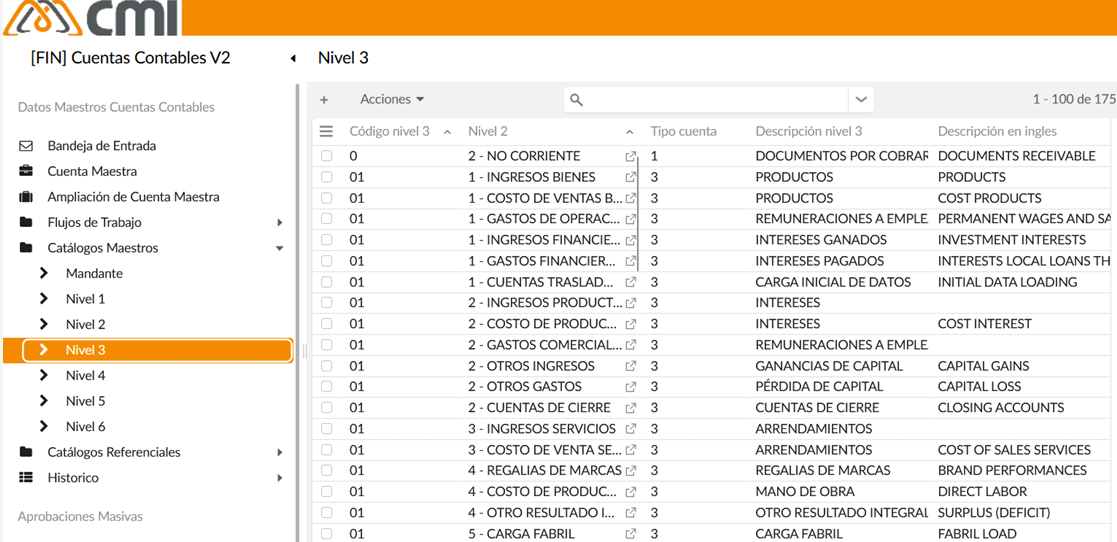
\includegraphics[width=0.8\textwidth]{RecorridoPerspectiva/ImgRecorridoPerspectiva/RP22.png}
     
    \end{minipage}

    \item
    \begin{minipage}[t]{\linewidth}
        Dentro de "Nivel 4" se encuentra el catálogo al cuarto nivel de una cuenta contable.
        
        \raggedright
        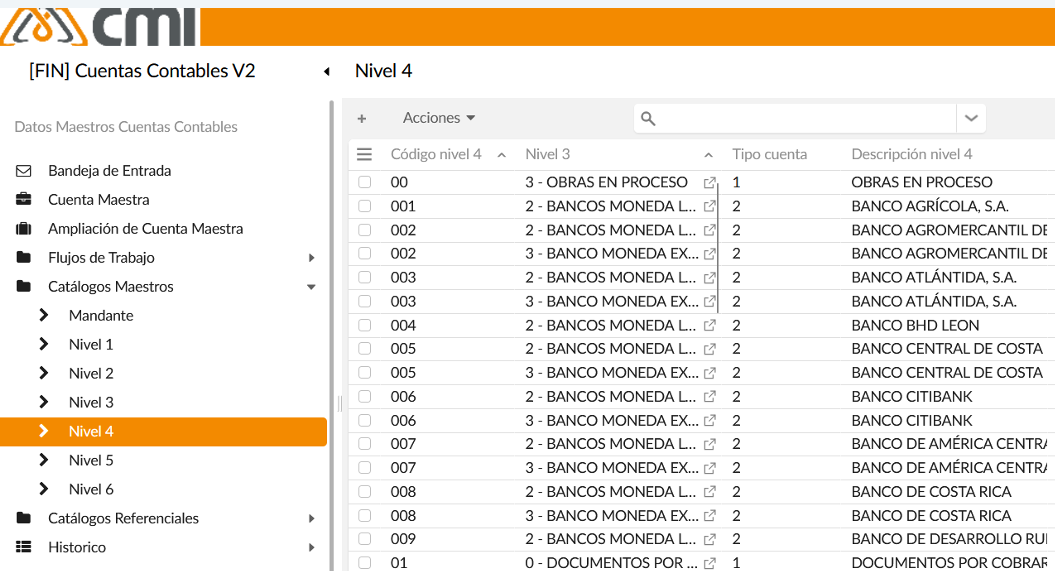
\includegraphics[width=0.8\textwidth]{RecorridoPerspectiva/ImgRecorridoPerspectiva/RP23.png}
     
    \end{minipage}

    \item
    \begin{minipage}[t]{\linewidth}
        Dentro de "Nivel 5" se encuentra el catálogo al quinto nivel de una cuenta contable.
        
        \raggedright
        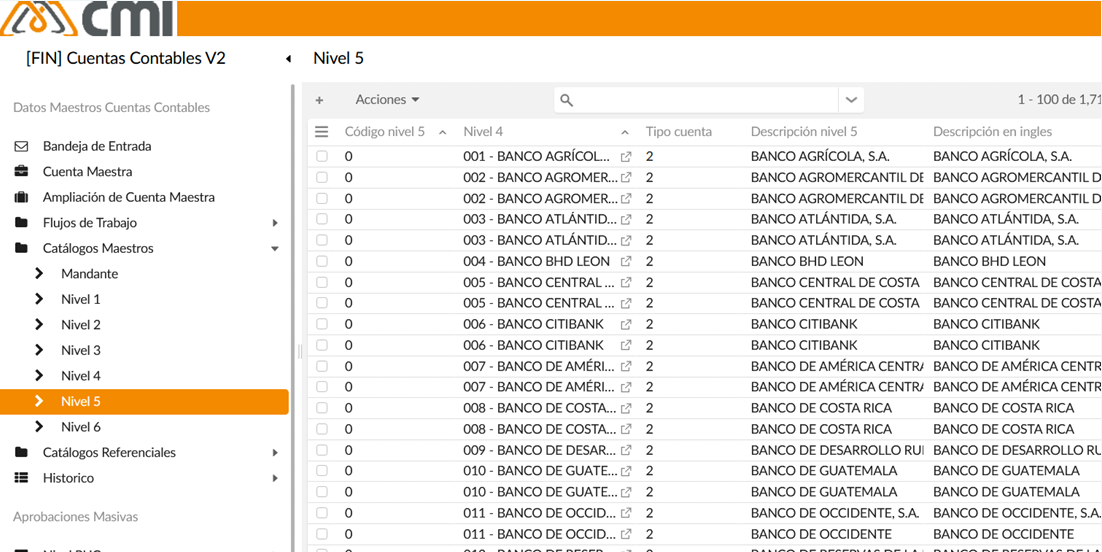
\includegraphics[width=0.8\textwidth]{RecorridoPerspectiva/ImgRecorridoPerspectiva/RP24.png}
     
    \end{minipage}

    \item
    \begin{minipage}[t]{\linewidth}
        Dentro de "Nivel 6" se encuentra el catálogo al sexto nivel de una cuenta contable.
        
        \raggedright
        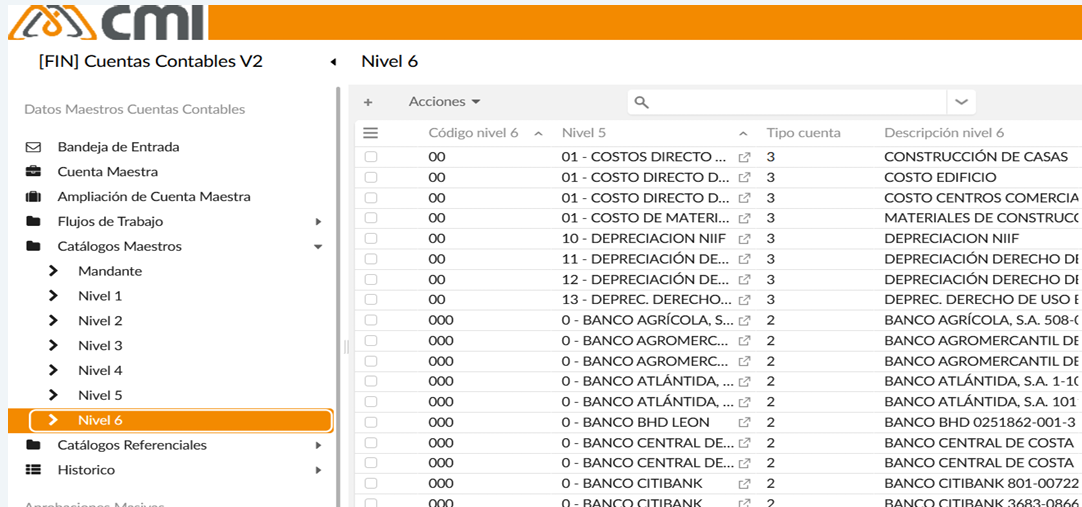
\includegraphics[width=0.8\textwidth]{RecorridoPerspectiva/ImgRecorridoPerspectiva/RP25.png}
     
    \end{minipage}


    \item
    \begin{minipage}[t]{\linewidth}
        Si damos click en "Parámetro y Valor".

        \raggedright
        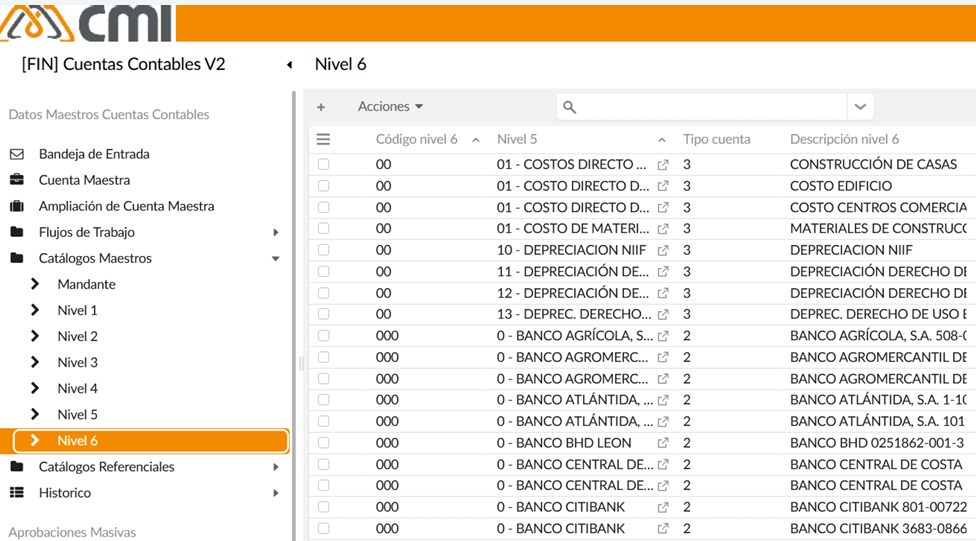
\includegraphics[width=0.8\textwidth]{RecorridoPerspectiva/ImgRecorridoPerspectiva/RP26.png}
     
    \end{minipage}
%%-----
    \item
    \begin{minipage}[t]{\linewidth}
        Si damos click en "Parámetro y Valor".

        \raggedright
        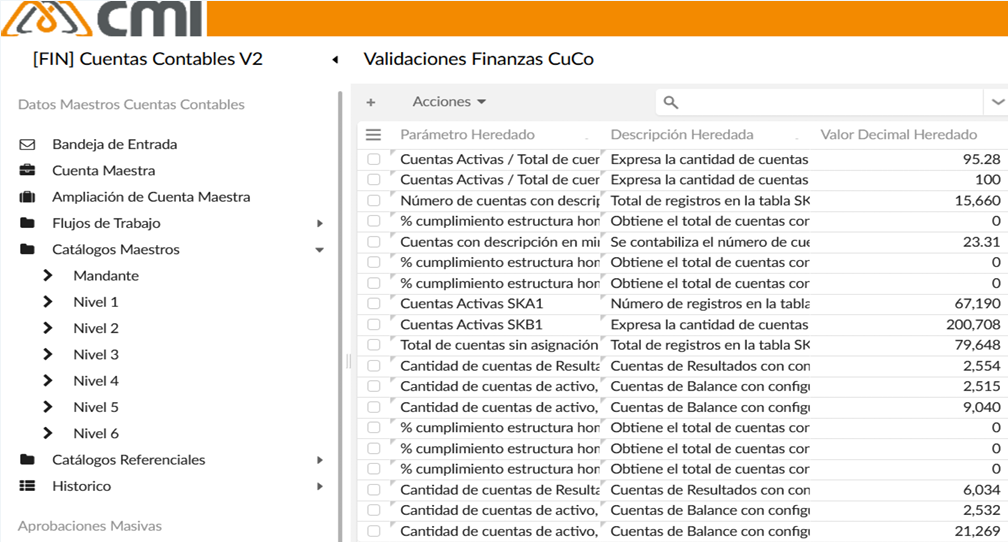
\includegraphics[width=0.8\textwidth]{RecorridoPerspectiva/ImgRecorridoPerspectiva/RP27.png}
     
    \end{minipage}

    \item
    \begin{minipage}[t]{\linewidth}
        Click "Parámetro y Valor".

        \raggedright
        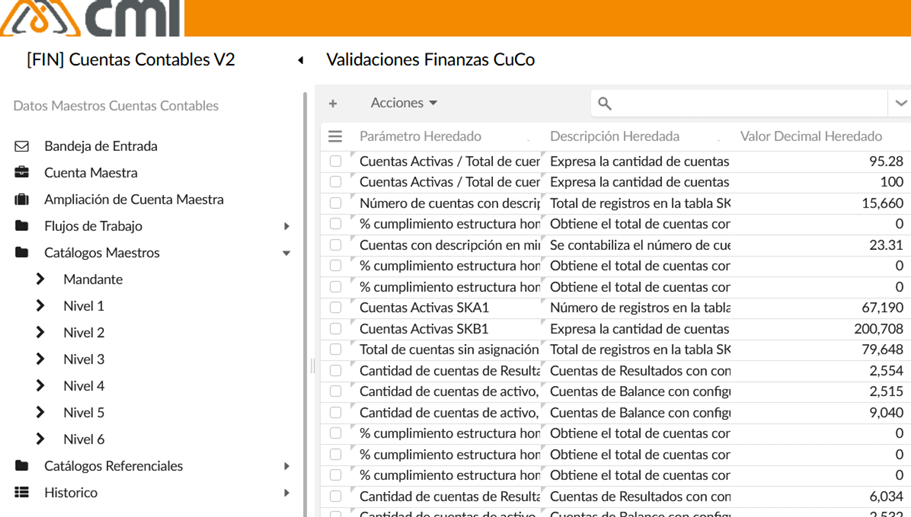
\includegraphics[width=0.8\textwidth]{RecorridoPerspectiva/ImgRecorridoPerspectiva/RP28.png}
     
    \end{minipage}

    \item
    \begin{minipage}[t]{\linewidth}
        Se muestra una tabla que contiene los resultados generales de las reglas de calidad.

        \raggedright
        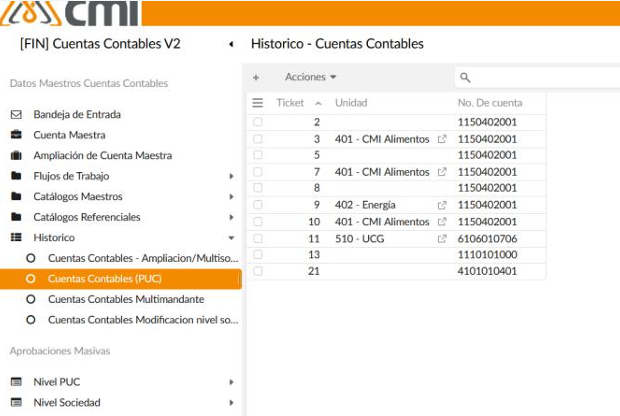
\includegraphics[width=0.8\textwidth]{RecorridoPerspectiva/ImgRecorridoPerspectiva/RP29.png}
     
    \end{minipage}

    \item
    \begin{minipage}[t]{\linewidth}
        En el apartado de Histórico se puede ver un espacio de registros y cambios realizados a una cuenta finalizada o en proceso. El área se divide en:

        \begin{itemize}
            \item Ampliación/Multi sociedad
            \item Nivel PUC
            \item Multi mandante
            \item Modificación a nivel sociedad
        \end{itemize}

        \raggedright
        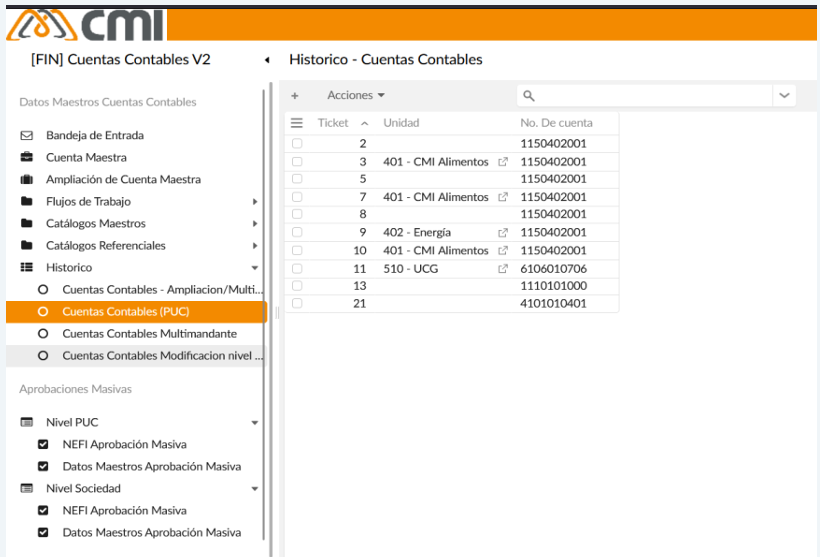
\includegraphics[width=0.6\textwidth]{RecorridoPerspectiva/ImgRecorridoPerspectiva/RP30.png}
     
    \end{minipage}

    \item
    \begin{minipage}[t]{\linewidth}
        En el área de Aprobaciones masivas se encuentran las tablas para procesos de funcionalidad Masiva, en su respectivo apartado se mostrará mejor su funcionamiento.

        \raggedright
        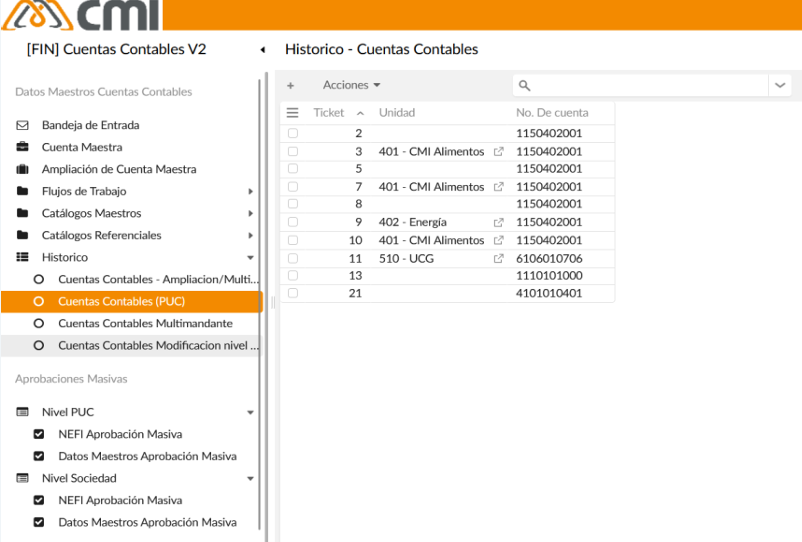
\includegraphics[width=0.8\textwidth]{RecorridoPerspectiva/ImgRecorridoPerspectiva/RP31.png}
     
    \end{minipage}





\end{enumerate}